\documentclass[12pt,fleqn]{article}\usepackage{../../common}
\begin{document}
Döndürme (Rotation)

Herhangi bir boyutta döndürme işlemi, yani bir noktayı ya da bir vektörün yönünü
değiştirmek lineer cebirsel bir matris çarpım işlemi üzerinden hesaplanabilir.
Daha önce [2]'de gördüğümüz baz değiştirme tekniği burada da geçerli. Baz
değiştirme de iki boyutta $i$,$j$, ya da $[0,1]$ ve $[1,0]$ vektörlerinin
yeni bir yöne işaret etmesi ve bu değişim sırasında ilk uzaydaki şeklin
bu değişimle beraber değişmesi olarak görülebilir. Bu yeni bazı kolonlarında
taşıyan şey ise bir nevi döndürme matrisi $R$'dir.

Eğer bir vektörü 90 derece saat yönü tersine döndürmek isteseydik, yeni baz
nasıl olurdu? $i$'yi kaldırıp tam yukarı işaret ettirmek lazım, o zaman
$[0,1]^T$, $j$ ise aynı şekilde sola yatırılmalı, $[-1, 0]$. Rotasyon matrisi,

$$
R = \left[\begin{array}{rr}
0 & -1 \\ 1 & 0
\end{array}\right]
$$


\begin{minted}[fontsize=\footnotesize]{python}
v = np.array([1,1])
plt.quiver(0,0,v[0],v[1],scale=5)
R = np.array([[0, -1],[1,0]])
vnew = np.dot(R, v)
plt.quiver(0,0,vnew[0],vnew[1],scale=5,color='red')
plt.xlim(-2,2)
plt.ylim(-2,2)
plt.grid(True)
plt.savefig('phy_072_rot_04.png')
\end{minted}

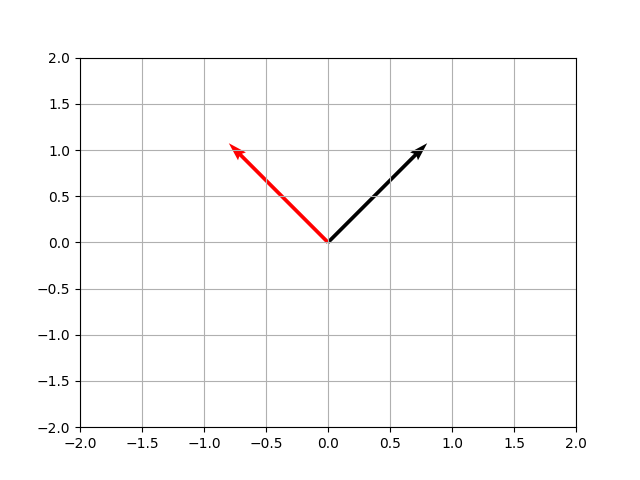
\includegraphics[width=20em]{phy_072_rot_04.png}

Doksan derece dönüş görülüyor.


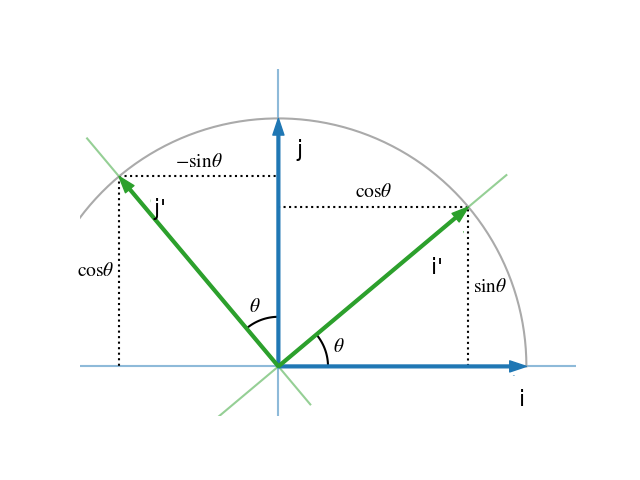
\includegraphics[width=20em]{phy_072_rot_03.png}



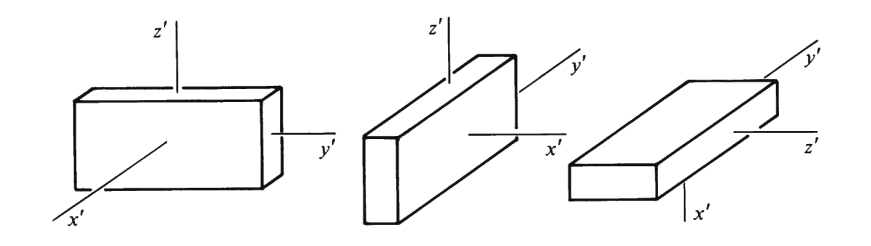
\includegraphics[width=20em]{phy_072_rot_01.png}

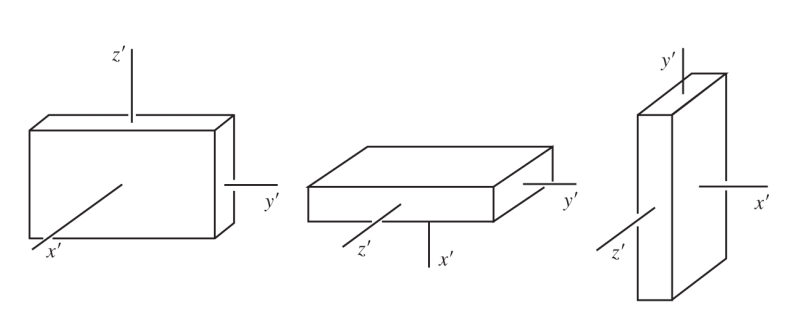
\includegraphics[width=20em]{phy_072_rot_02.png}












Kaynaklar

[1] Safko, {\em Classical Mechanics}

[2] Bayramli, {\em Lineer Cebir, Giris}

\end{document}

